\section{Frontend}
Webová aplikace je primárně postavena na Vue.js, moderní JavaScriptové knihovně určené k tvorbě dynamických uživatelských rozhraní. Využívá komponentový přístup, který umožňuje rozdělit rozhraní na menší, znovu použitelné části, čímž usnadňuje správu kódu a zlepšuje čitelnost projektu. Tento přístup nejen zjednodušuje vývoj, ale také usnadňuje rozšiřování a údržbu aplikace, což je klíčové pro škálovatelnost projektu.
\subsection{Routování}
V Nuxtu funguje routování automaticky díky file-based routing, což znamená, že struktura souborů ve složce \textit{pages/} určuje URL adresy aplikace. Například soubor \textit{pages/index.vue} odpovídá domovské stránce \textit{/}, zatímco \textit{pages/about.vue} vytváří routu \textit{/about}. Pro dynamické parametry se používají hranaté závorky, takže soubor \textit{pages/blog/[id].vue} odpovídá cestě \textit{/blog/:id}, kde lze parametr id získat pomocí \textit{useRoute()}.\cite{routing}
\subsection{Komponenty}
Vue.js i Nuxt staví na technologii komponentů.
Komponenty umožňují rozdělit komplexní UI problémy do mnoha menších podproblémů; je to podobné jako například funkce nebo třídy v objektově orientovaném programování. Jednotlivé komponenty jsou samostatné .vue soubory ve složce \textit{components}, obsahují HTML šablony, JavaScriptový (popřípadě TypeScriptový) kód i CSS styly. Komponenty pomáhají modulárně strukturovat aplikaci, což vede k lepší čitelnosti a opětovné použitelnosti kódu.\cite{component} Dále bych chtěl podotknout, že Nuxt zajišťuje automatické importování komponent, není tedy potřeba je v každém souboru importovat manuálně. \cite{nuxt-auto-import}
\newline
\newline
Nejvýznamnějším komponentem v tomto projektu je \textit{MapNetwork.vue}. V tomto komponentu se do hromady skládá veškerá funkcionalita nástroje na tvorbu myšlenkových map. V jádru této komponenty stojí knihovna V-network-graph, která se stará o reprezentaci i zobrazování relačních grafů viz kapitola \ref{vizualizcemap}. Jsou zde napojeny další UI komponenty, jak funkce spravující grafovou strukturu, tak funkce dotazující do databáze. Dále jsou zde handlery na obsluhování klávesových zkratek.
\newline
Dalšími významnými komponenty jsou \textit{NodeInputDialog.vue} \textit{NodeEditDialog.vue}, tyto UI komponenty zprostředkovávají uživatelské rozhraní pro editace (případně tvorbu) jednotlivých nodů. 

\subsection{Design}
Idea-Atlas je proveden v jednoduchém, čistém stylu. Dominantními barvami jsou modrá, světle šedá a bílá. Snažil jsem se, aby uživatelské rozhraní působilo přehledně a moderně, ale nikoliv však rušivě. Schválně jsem se vyhnul komplikovaným designovým prvkům a animacím, protože to není předmětem této práce.
\par
Zde jsou vyobrazeny ukázky těch zajímavějších částí webové aplikace. Na obrázku \ref{fig:home} je k nalezení hero nadpis úvodní domovské stránky. Na něm bych vypíchnul minimalistický design pomocí gradientů a poklidnou jednoduchou animaci pohupování.\cite{glow}
\begin{figure}[h]
    \centering
    
\includegraphics[width=0.9\linewidth]{Images/Homepage.png}
    \caption{Hero nadpis}
    \label{fig:home}
\end{figure}
\newpage
Na obrázku \ref{fig:card} je k vidění kartička jedné z map. Je na ní vidět, zda je bookmarknutá, kdy byla mapa vytvořena, kdy naposledy upravena, její jméno a popis.\cite{card} Dále jsou zde ikonky pro smazání dané mapy nebo upravení jejích metadat.
\begin{figure}[h]
    \centering
    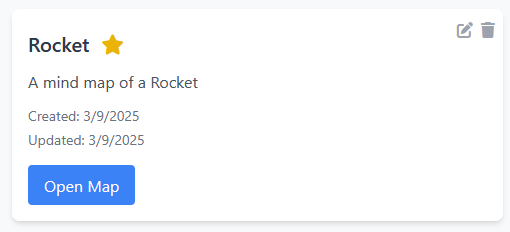
\includegraphics[width=1\linewidth]{Images/card.png}
    \caption{Kartička mapy}
    \label{fig:card}
\end{figure}
